% Short version of "A Symbolic-Free Affine Arithmetic with Zero-Centered Residuals"
% prepared for Optimization Letters (~15 journal pages).
% The page layout below approximates the Springer journal text block
% (10pt Times, 122 x 198 mm) so that the page count is representative.
% For the actual submission, the content can be moved to Springer's sn-jnl class.
\documentclass[10pt]{article}
\usepackage[paperwidth=155mm,paperheight=235mm,textwidth=122mm,textheight=198mm,centering]{geometry}
\usepackage{mathptmx}
\usepackage{graphicx}
\usepackage{amsmath}
\usepackage{amsthm}
\usepackage{booktabs}
\usepackage{url}
\usepackage{intmacros}

\newcommand{\Rset}{\mathbb{R}}
\newcommand{\IRset}{\mathbb{IR}}
\newcommand{\midp}{\mathrm{mid}}
\renewcommand{\wid}{\mathrm{wid}}

\newtheorem{propo}{Proposition}
\newtheorem{remark}{Remark}

\title{A Symbolic-Free Affine Arithmetic with Zero-Centered Residuals}
\author{Ignacio Araya \and Angelo Alvear Tapia \and Daniel Miranda \and Juan Aramayo \and Victor Reyes}
\date{}

\begin{document}
\maketitle

\begin{abstract}
Affine arithmetic is widely used to compute range enclosures and linear relaxations of factorable functions, but in its classical variants the offsets of the nonlinear residuals are kept in symbolic noise terms and accumulate through successive multiplications. We introduce a zero-centered affine arithmetic (ZCAA) in which each subexpression is represented by a linear function of the original variables plus a bounded residual interval, without symbolic noise variables. At each multiplication, the midpoints of the residuals of the operands are absorbed into the linear coefficients, so that the residuals propagated to the next operations are centered at zero. We prove that ZCAA coincides with the AF2 variant of affine arithmetic on products of affine expressions, and that zero-centered residuals minimize the width propagated through a product. On controlled expressions and on constraints from a benchmark of nonlinear systems, ZCAA is never looser than AF2 or first-order Taylor models; on the controlled products, its residual width is smaller than that of AF2 by 5.6\% on average and by up to 46\%, and smaller than that of Taylor models by 1.5\% on average and by up to 25\%, mostly in wide boxes.

\medskip\noindent
\textit{Keywords:} affine arithmetic, interval arithmetic, range enclosure, linear relaxation, global optimization
\end{abstract}

\section{Introduction}

Branch-and-bound (B\&B) solvers for global optimization evaluate range enclosures and linear relaxations of the constraints and of the objective function at every node, often millions of times, so these routines must be both tight and fast. Interval arithmetic (IA)~\cite{moore1966} is the simplest way to obtain enclosures, but it suffers from the dependency problem. Affine arithmetic (AA)~\cite{combastolfi1993} keeps the linear dependencies between quantities through symbolic noise variables, and its affine forms provide, in addition to an enclosure, a pair of parallel linear under- and over-estimators that can be embedded in B\&B solvers~\cite{ninin2015reliable,araya2025hybridizing}. Each nonlinear operation of standard AA introduces a new noise symbol; the variants AF1 and AF2~\cite{messine2002extentions} keep the number of symbols fixed by accumulating the nonlinear errors in one symmetric term (AF1) or in a symmetric and two one-sided terms (AF2), the latter capturing, e.g., the nonnegativity of squares. Other extensions include second-order terms~\cite{LIAO2020105440,messine2006general}, a redistribution of the multiplication error over existing symbols~\cite{kumar}, an optimal $O(n)$ bound of the multiplication error for reduced affine forms~\cite{skalna2017new}, and refined divisions~\cite{jacquemin2019dividing}.

The representation used here, a linear function of the variables plus an interval remainder, is that of first-order Taylor models (TM)~\cite{makino2003}, a variant of centered forms~\cite{neumaier2003taylor}. In a TM of order~1, the product of $(P_1, I_1)$ and $(P_2, I_2)$ encloses the whole second-order part of $P_1P_2$ in one interval and the cross terms as $B(P_1) I_2 + B(P_2) I_1 + I_1 I_2$, where $B(P)$ bounds $P$ over the box~\cite[Def.~2]{makino2003}; the remainders are not re-centered. In AF2, the one-sided terms $\epsilon_+$ and $\epsilon_-$ have nonzero midpoints, and these offsets are carried along through the next products.

\paragraph{Contributions.} We propose a \emph{zero-centered affine arithmetic} (ZCAA) that combines the two ideas: (i) as in AF2, every quadratic and bilinear monomial generated by a product is enclosed by its own linear envelope, and (ii) the midpoints of the residuals of the operands are absorbed into the linear coefficients before the cross terms are bounded, so that every residual propagated through the expression tree is centered at zero. The bounds of the residual of a product are computed exactly by evaluating four linear functions over the box. We prove that ZCAA and AF2 coincide on products of purely affine expressions (Proposition~\ref{prop:af2}) and that a zero-centered residual minimizes the width propagated through a product (Proposition~\ref{prop:center}). Experiments on controlled expressions and on constraints of a standard benchmark show that ZCAA is never looser than AF2 or TM, and is strictly tighter whenever the operands carry residuals.

\section{Zero-centered affine arithmetic}
\label{sec:zcaa}

\paragraph{Notation.} An interval $\x_i=[\ul x_i,\ol x_i]$ has width $\wid(\x_i)=\ol x_i-\ul x_i$ and midpoint $\midp(\x_i)=(\ul x_i+\ol x_i)/2$; a box $\x=\x_1\times\dots\times\x_n$ is a vector of intervals. For reference, an AF2 form is $\hat x=a_0+\sum_{i=1}^n a_i\epsilon_i+a_\pm\epsilon_\pm+a_+\epsilon_++a_-\epsilon_-$ with $\epsilon_i,\epsilon_\pm\in[-1,1]$, $\epsilon_+\in[0,1]$, $\epsilon_-\in[-1,0]$ and $a_\pm,a_+,a_-\ge 0$~\cite{messine2002extentions}; in a product, the squares $\epsilon_i^2$ are accumulated in $\epsilon_+$, the bilinear terms $\epsilon_i\epsilon_j$ in $\epsilon_\pm$, and the products involving the error terms in $\epsilon_\pm$, $\epsilon_+$ or $\epsilon_-$ according to their signs.

\paragraph{Representation.} In ZCAA, every subexpression $v$ is represented by
\begin{equation}
\label{eq:form}
\hat v(x)=\sum_{i=1}^n a_i x_i + r_v,\qquad x\in\x,\ r_v\in\r_v,
\end{equation}
where $a\in\Rset^n$ and $\r_v$ is an interval that contains the intercept and bounds the deviation of $v$ from its linear part over $\x$. The lines $\sum a_ix_i+\ul r_v$ and $\sum a_ix_i+\ol r_v$ are valid linear under- and over-estimators of $v$, and $\wid(\r_v)$, the vertical distance between them, measures the quality of the relaxation. The variables are $\hat x_i = x_i + [0,0]$. Sums and products by scalars are exact: $\hat v+\hat w=\sum(a_i+b_i)x_i+(\r_v+\r_w)$ and $\lambda\hat v=\sum\lambda a_ix_i+\lambda\r_v$.

\paragraph{Univariate functions.} For $u(\hat v)$ with $u$ convex or concave over the range $\vv=[\ul v,\ol v]$ of $\hat v$, we use the Chebyshev slope $m=(u(\ol v)-u(\ul v))/(\ol v-\ul v)$ and set $\hat u=m\hat v+\r_u$ with $\r_u=[\min_{v\in\vv}g(v),\max_{v\in\vv}g(v)]$, $g(v)=u(v)-mv$, whose extrema are attained at the endpoints of $\vv$ or at the solution of $u'(v)=m$. This is the classical minimax linearization of AA~\cite{stolfi1997self}. For instance, $\widehat{x_i^2}=(\ul x_i+\ol x_i)\,x_i+[-\midp(\x_i)^2,\,-\ul x_i\ol x_i]$.

\subsection{Bilinear monomials}
\label{sec:bilinear}

For $x_ix_j$ over $\x_i\times\x_j$, we take the tangent plane at the center of the box, with slopes $m_i=\midp(\x_j)$ and $m_j=\midp(\x_i)$. With $x_i=m_j+\delta_i$ and $x_j=m_i+\delta_j$, the residual is $x_ix_j-m_ix_i-m_jx_j=\delta_i\delta_j-m_im_j$, where $|\delta_i|\le\wid(\x_i)/2$ and $|\delta_j|\le\wid(\x_j)/2$ vary independently, so that
\begin{equation}
\label{eq:bilinear}
\widehat{x_ix_j}=m_ix_i+m_jx_j+\left[-\tfrac{\wid(\x_i)\wid(\x_j)}{4},\ \tfrac{\wid(\x_i)\wid(\x_j)}{4}\right]-m_im_j,
\end{equation}
and this residual interval is exact. The McCormick envelopes~\cite{mccormick1976}, the maximum and minimum of two planes, are tighter, but the parallel pair keeps the result in the form~\eqref{eq:form}, so that it can be propagated through further operations.

\subsection{Product of two affine forms}
\label{sec:product}

Let $\hat v=\sum a_ix_i+r_v$ and $\hat w=\sum b_ix_i+r_w$. Their product is
\begin{equation}
\label{eq:expanded}
\hat v\hat w=\sum_i a_ib_i x_i^2+\sum_{i<j}(a_ib_j+a_jb_i)x_ix_j + r_v\sum_i b_ix_i + r_w\sum_i a_ix_i + r_vr_w.
\end{equation}
We write each residual as its midpoint plus a zero-centered deviation, $r_v=\dot r_v+\delta_v$ and $r_w=\dot r_w+\delta_w$, with $\dot r_v=\midp(\r_v)$ and $\dot r_w=\midp(\r_w)$. The deterministic part $\dot r_w\sum a_ix_i+\dot r_v\sum b_ix_i$ of the cross terms is linear and is absorbed into the linear coefficients, and the remaining residual is
\begin{equation}
\label{eq:ru}
r(x,r_v,r_w)=\sum_i(\delta_w a_i+\delta_v b_i)\,x_i+r_vr_w .
\end{equation}
For a fixed $x$, $r$ is bilinear in $(r_v,r_w)$, so its extrema over $\r_v\times\r_w$ are attained at the four vertices $V_r=\{\ul r_v,\ol r_v\}\times\{\ul r_w,\ol r_w\}$. For each vertex, $r$ is a linear function of $x$, whose exact range over $\x$ is given by its natural interval extension. Hence
\begin{equation}
\label{eq:Rbounds}
\r = \Big[\min_{V_r}\ \min_{x\in\x} r,\ \max_{V_r}\ \max_{x\in\x} r\Big]
\end{equation}
is the exact range of~\eqref{eq:ru} over $\x\times\r_v\times\r_w$, and is computed in $O(n)$ operations. Replacing each monomial of~\eqref{eq:expanded} by its enclosure gives the ZCAA product
\begin{equation}
\label{eq:zcaa-product}
\widehat{v\cdot w}=\sum_i(\dot r_wa_i+\dot r_vb_i)\,x_i+\sum_i a_ib_i\,\widehat{x_i^2}+\sum_{i<j}(a_ib_j+a_jb_i)\,\widehat{x_ix_j}+\r ,
\end{equation}
which is again of the form~\eqref{eq:form}. If $\hat v$ and $\hat w$ have at most $n$ nonzero coefficients and their expansion has $m\le n(n+1)/2$ quadratic and bilinear monomials, the product takes $O(n+m)$ operations, since the envelopes of the monomials over $\x$ are computed once per box in $O(1)$ each. This is the same order as the AF2 product of~\cite{messine2002extentions}, which also treats each monomial $\epsilon_i\epsilon_j$ separately.

\paragraph{Example.} Let $\hat v=x_1+2x_2+[-1,1]$ and $\hat w=2x_1+3x_2+[0,2]$ over $x_1,x_2\in[0,2]$, i.e., $\hat v=3+\epsilon_1+2\epsilon_2+\epsilon_\pm$ and $\hat w=5+2\epsilon_1+3\epsilon_2+2\epsilon_+$ in AF2. In ZCAA, $\dot r_v=0$ and $\dot r_w=1$, so the absorbed linear part is $x_1+2x_2$. The quadratic monomials give $2\widehat{x_1^2}+6\widehat{x_2^2}=4x_1+12x_2+[-8,0]$, and the bilinear one gives $7\widehat{x_1x_2}=7x_1+7x_2+[-14,0]$. The residual~\eqref{eq:ru} evaluated at the four vertices ranges in $[-16,0]$, $[-2,2]$, $[0,4]$ and $[2,18]$, so $\r=[-16,18]$, and
\[
\widehat{v\cdot w}=12x_1+21x_2+[-38,18].
\]
AF2 gives $15+11\epsilon_1+19\epsilon_2+14\epsilon_++25\epsilon_\pm$, i.e., $11x_1+19x_2+[-40,24]$. The enclosures of the monomials coincide, and the difference in thickness (56 versus 64) comes entirely from the cross terms: AF2 multiplies the offset $2\epsilon_+$ of $\hat w$ by the whole form $\hat v$ and stores the result in its error terms.

\section{Properties}
\label{sec:properties}

The first result states that ZCAA brings nothing new when the operands carry no residual; its proof (Online Resource~1) shows that the ZCAA and AF2 enclosures of $x_i^2$ and $x_ix_j$ coincide after the substitution $\epsilon_i=(x_i-\midp(\x_i))/(\wid(\x_i)/2)$, and that the AF2 enclosure of a product of linear forms is the sum of the AF2 enclosures of its monomials.

\begin{propo}
\label{prop:af2}
Let $f(x)=\sum_i a_ix_i$ and $g(x)=\sum_i b_ix_i$ with $x\in\x$. Then the ZCAA and AF2 enclosures of $f\cdot g$ coincide.
\end{propo}

When the operands carry residuals, the two methods differ only in the cross terms $L_v(x)\,r_w$ and $L_w(x)\,r_v$ of~\eqref{eq:expanded}, where $L_v$ and $L_w$ are the linear parts. Over $\x$, $L_v(x)$ ranges in an interval $\y$, so the uncertainty contributed by $L_v(x)\,r_w$ is that of the interval product $\r_w\cdot\y$. The next result shows that, for a given width of the residual, centering it at zero, as ZCAA does at every multiplication, minimizes the width of this product.

\begin{propo}
\label{prop:center}
Let $\y=[\ul y,\ol y]$ be an interval, $\rho\ge 0$ and $Y=\max(|\ul y|,|\ol y|)$. Among all the intervals $\r=[r_c-\rho,\,r_c+\rho]$, $r_c\in\Rset$, the width of $\r\cdot\y$ attains its minimum $2\rho Y$ at $r_c=0$.
\end{propo}

\begin{proof}
Let $y^*\in\{\ul y,\ol y\}$ with $|y^*|=Y$. For every $r_c$, $\r\cdot\y$ contains $(r_c-\rho)y^*$ and $(r_c+\rho)y^*$, whose distance is $2\rho Y$, so $\wid(\r\cdot\y)\ge 2\rho Y$. If $r_c=0$, then $|ry|\le\rho Y$ for all $r\in\r$ and $y\in\y$, and $\pm\rho y^*\in\r\cdot\y$, so $\r\cdot\y=[-\rho Y,\rho Y]$.
\end{proof}

The minimizer need not be unique: if $\y\subseteq[0,\infty)$, every $\r$ that contains zero gives the same width. Proposition~\ref{prop:center} does not imply that ZCAA is tighter than AF2 on every expression, but it explains the mechanism observed in the example and in the experiments: AF2 keeps the offsets of $\epsilon_+$ and $\epsilon_-$ inside the error terms, where they are multiplied by the whole range of the other factor, whereas ZCAA moves them to the linear part, where they are represented exactly.

\section{Experiments}
\label{sec:experiments}

ZCAA, AF2~\cite{messine2002extentions} and first-order TM~\cite{makino2003} were implemented in a Python prototype with floating-point arithmetic, without outward rounding; the enclosures were checked by evaluating the expressions at random points of each box. In TM, the second-order part of a product is enclosed monomial by monomial, so that the squares $(x_i-\midp(\x_i))^2$ are enclosed in $[0,\wid(\x_i)^2/4]$, and the remainders are combined as in~\cite[Def.~2]{makino2003}. The three methods use the same Chebyshev linearization for the univariate functions, so that the differences come only from the multiplications. Code, data and scripts are available at \url{https://github.com/rilianx/raa-affine-arithmetic}.

We measure the width $W_M$ of the residual of each method $M$, i.e., the thickness of its relaxation ($2a_\pm+a_++a_-$ in AF2), and report the gap $100\,(W_M-W_{\mathrm{OPT}})/W_{\mathrm{OPT}}$, where $W_{\mathrm{OPT}}$ is the exact width of the range of $f(x)-f_l(x)$ over the box, $f_l$ being the linear part of the ZCAA form, computed with IbexOpt~\cite{chabert2009}. Since the reference is the same for the three methods, differences between gaps are proportional to differences between thicknesses.

\paragraph{Controlled expressions.} We consider four products in three variables: Case~1, $(x_1+2x_2+3x_3)(4x_1+5x_2+6x_3)$ (affine operands); Case~2, $(x_1+2x_2^2+3x_3)(4x_1+5x_2+6x_3^2)$ (quadratic residuals); Case~3, $(x_1+2x_2x_3)(3x_2+4x_1x_3)$ (bilinear residuals); and Case~4, $(x_1+2x_2)(3x_2+4x_3)(5x_3+6x_1)$ (chained products). In an AA evaluation, every multiplication node combines two subexpressions already reduced to affine forms with residuals, so these patterns occur at the inner nodes of general expression trees. For each case, 100 boxes are sampled in $[-10,10]^3$ with widths in $[0.01,0.1]$ (S), $[0.1,1]$ (M) or $[1,10]$ (L).

\begin{table}[t]
\centering
\caption{Gaps (\%) with respect to the optimal residual width, mean $\pm$ standard deviation over 100 boxes, and median $[P_{10},P_{90}]$ of the run-by-run difference between the gaps of AF2 and ZCAA.}
\label{tab:controlled}
\small
\setlength{\tabcolsep}{3.5pt}
\begin{tabular}{llrrrr}
\toprule
Case & Size & TM & AF2 & ZCAA & AF2$-$ZCAA \\
\midrule
1 & S & $58.18 \pm 5.93$ & $58.18 \pm 5.93$ & $58.18 \pm 5.93$ & $0.00\ [0.00, 0.00]$ \\
  & M & $58.10 \pm 5.62$ & $58.10 \pm 5.62$ & $58.10 \pm 5.62$ & $0.00\ [0.00, 0.00]$ \\
  & L & $55.62 \pm 7.51$ & $55.62 \pm 7.51$ & $55.62 \pm 7.51$ & $0.00\ [0.00, 0.00]$ \\
\midrule
2 & S & $40.82 \pm 13.15$ & $46.40 \pm 16.93$ & $40.78 \pm 13.13$ & $2.95\ [0.00, 13.71]$ \\
  & M & $42.61 \pm 10.89$ & $48.31 \pm 13.71$ & $42.13 \pm 10.81$ & $3.92\ [0.02, 14.12]$ \\
  & L & $48.49 \pm 14.86$ & $52.48 \pm 17.44$ & $42.46 \pm 12.60$ & $6.09\ [0.79, 22.87]$ \\
\midrule
3 & S & $31.75 \pm 11.30$ & $43.17 \pm 23.62$ & $31.66 \pm 11.27$ & $3.46\ [0.00, 31.29]$ \\
  & M & $34.36 \pm 13.93$ & $45.17 \pm 29.01$ & $33.12 \pm 12.60$ & $3.44\ [0.02, 30.65]$ \\
  & L & $34.11 \pm 15.51$ & $39.19 \pm 20.09$ & $22.81 \pm 11.49$ & $12.44\ [3.03, 31.65]$ \\
\midrule
4 & S & $76.74 \pm 82.49$ & $81.61 \pm 82.28$ & $76.74 \pm 82.49$ & $0.10\ [0.02, 17.90]$ \\
  & M & $98.27 \pm 87.17$ & $105.75 \pm 91.83$ & $98.27 \pm 87.17$ & $0.99\ [0.15, 26.03]$ \\
  & L & $77.78 \pm 38.59$ & $89.70 \pm 43.02$ & $76.52 \pm 39.07$ & $10.32\ [1.53, 27.13]$ \\
\bottomrule
\end{tabular}
\end{table}

Table~\ref{tab:controlled} summarizes the results. In Case~1, the three methods coincide, as predicted by Proposition~\ref{prop:af2}. In Cases~2--4, ZCAA is tighter than AF2 in all the 900 runs (Fig.~\ref{fig:scatter}) (one-sided Wilcoxon signed-rank test over the 1200 runs, ties excluded, $p=3.4\times10^{-149}$) and is never looser. Its residual width is smaller than that of AF2 by 5.6\% on average (median 3.0\%, 90th percentile 14.8\%, maximum 46.0\%), and the advantage grows with the size of the box. TM avoids most of the overestimation of AF2: it is tighter than AF2 in 693 of the 900 runs and looser in 27. ZCAA is never looser than TM and is tighter in 623 of the 1200 runs ($p=5.3\times10^{-104}$); its residual width is smaller by 1.5\% on average (maximum 24.9\%), with a 90th percentile of 0.1\%, 0.9\% and 11.4\% in small, medium and large boxes. The advantage over TM thus comes from the re-centering of the remainders and is noticeable mainly in wide boxes.

\begin{figure}[t]
\centering
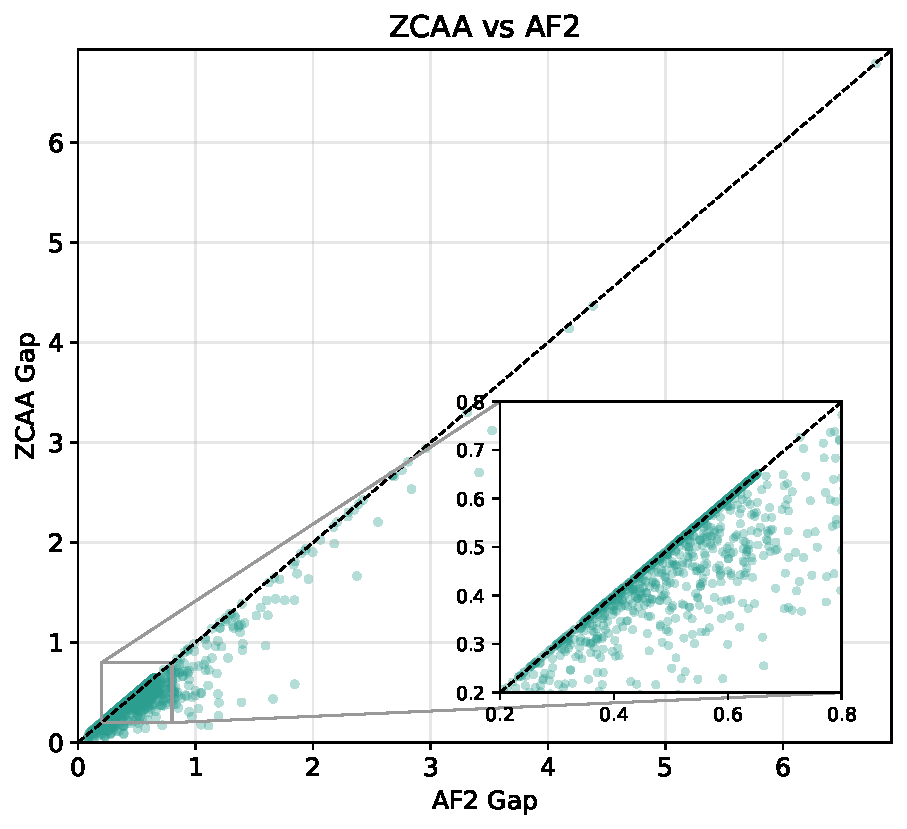
\includegraphics[width=0.75\linewidth]{Fig2.pdf}
\caption{Gap of ZCAA against gap of AF2 for the 1200 runs of the controlled expressions. Points below the diagonal are runs where ZCAA is tighter.}
\label{fig:scatter}
\end{figure}

\paragraph{Constraints from a benchmark.} We searched the 222 systems of a benchmark of nonlinear systems~\cite{coprin} for products whose two factors depend on at least two variables. Most of them multiply two affine factors, for which ZCAA and AF2 coincide (Proposition~\ref{prop:af2}). We selected four constraints in three variables whose products have nonlinear factors:
Trigexp1 (2nd constraint), $-8+\sin(x_2-x_3)\sin(x_2+x_3)-e^{x_1-x_2}x_1-4x_2+3x_2^3+2x_3$;
Trigexp2 (1st), $-5+\sin(x_1-x_2-x_3)\sin(x_1+x_2-x_3)+2x_2+3(x_1-x_3)^3$;
Trigexp2 (2nd), $-3+4x_2-e^{x_1-x_2-x_3}(x_1-x_3)$;
and Pramanik (1st), a sum of three squared polynomials of degree up to four built from nested products. Boxes are sampled in $[-10,10]^3$ for Trigexp and in the domain $[0.06,1]^3$ of Pramanik (small and medium boxes only), with 100 runs per size for Trigexp1 and 50 for the others.

\begin{table}[t]
\centering
\caption{Benchmark constraints: mean gaps (\%) and mean reduction of the residual width of ZCAA with respect to TM and AF2 (\%).}
\label{tab:instances}
\small
\begin{tabular}{llrrrrr}
\toprule
 & & \multicolumn{3}{c}{Gap (\%)} & \multicolumn{2}{c}{Red. of ZCAA (\%)} \\
\cmidrule(lr){3-5}\cmidrule(lr){6-7}
Constraint & Size & TM & AF2 & ZCAA & vs TM & vs AF2 \\
\midrule
Trigexp1 & S & 31.04 & 35.55 & 30.98 & 0.0 & 2.9 \\
 & M & 25.52 & 31.34 & 24.43 & 0.8 & 3.9 \\
 & L & 58.09 & 58.19 & 57.62 & 0.3 & 0.4 \\
\midrule
Trigexp2 (1) & S & 12.88 & 18.12 & 12.68 & 0.1 & 3.3 \\
 & M & 8.58 & 11.76 & 7.57 & 0.8 & 3.1 \\
 & L & 0.41 & 0.42 & 0.33 & 0.1 & 0.1 \\
\midrule
Trigexp2 (2) & S & 125.09 & 125.09 & 125.09 & 0.0 & 0.0 \\
 & M & 116.84 & 116.84 & 116.84 & 0.0 & 0.0 \\
 & L & 90.61 & 90.61 & 90.61 & 0.0 & 0.0 \\
\midrule
Pramanik & S & 360.61 & 363.34 & 360.61 & 0.0 & 0.6 \\
 & M & 693.08 & 700.15 & 693.08 & 0.0 & 0.9 \\
\bottomrule
\end{tabular}
\end{table}

Table~\ref{tab:instances} shows that ZCAA is again never looser than AF2 or TM, and tighter than AF2 in 549 of the 700 runs (significant for Trigexp1, Trigexp2~(1) and Pramanik, $p\le 1.9\times10^{-18}$). The gains are smaller than on the controlled products: 2.9--3.9\% with respect to AF2 in small and medium boxes of Trigexp, less than 0.5\% in large boxes, where the sine is linearized with a slope close to zero, and less than 1\% in Pramanik, where the linearization errors of the nested products dominate. In Trigexp2~(2), the second factor has no residual and the residual of the exponential is already centered in both methods, so the enclosures coincide. With respect to TM, ZCAA is tighter in 492 of the 700 runs ($p=1.3\times10^{-82}$), by at most 0.8\% on average per configuration.

\paragraph{Running time.} In the Python prototype, one evaluation of the controlled expressions takes 0.016--0.024\,ms with ZCAA, 0.016--0.020\,ms with AF2 and 0.015--0.035\,ms with TM; ZCAA takes 0.97--1.33 times the time of AF2 on the controlled expressions and 0.98--1.30 times on the benchmark constraints. These timings indicate relative cost only; a compiled implementation with outward rounding is needed to assess ZCAA inside a B\&B solver.

\section{Conclusion}

ZCAA represents every subexpression as a linear function of the variables plus a residual interval, encloses each quadratic and bilinear monomial of a product with its own envelope, and re-centers the residuals at every multiplication. It coincides with AF2 on products of affine forms, and the re-centering minimizes the width propagated through each product. Experimentally, ZCAA is never looser than AF2 or first-order Taylor models; it is noticeably tighter than AF2 whenever the operands carry residuals, and tighter than Taylor models mainly in wide boxes, at a cost comparable to AF2. Future work includes a compiled, rounding-safe implementation integrated into a B\&B solver, and envelopes with non-parallel lower and upper slopes.

\section*{Statements and declarations}
\textbf{Funding.} ANID, Chile, FONDECYT Regular 2026, project No.~1260159.
\textbf{Competing interests.} The authors have no relevant financial or non-financial interests to disclose.
\textbf{Data availability.} Code, data and scripts: \url{https://github.com/rilianx/raa-affine-arithmetic}.
\textbf{Use of AI.} The authors used an AI assistant (Claude, Anthropic) to help implement and verify the experimental code, run the experiments and check the proofs; all code, results and proofs were reviewed by the authors, who take full responsibility for them.
\textbf{Supplementary information.} Online Resource~1 contains the proof of Proposition~\ref{prop:af2}.

\bibliographystyle{unsrt}
\bibliography{bibliography}

\end{document}
